\section{Introduction}
Microphone arrays enable the acquisition of the space-time structure of an acoustic field. Thus they have been widely used to solve many tasks in computational auditory scene analysis such as source separation, source localization and tracking.
Systems that combine microphone arrays with a digital camera are getting more and more used for many applications.
For example, these systems are used for generating acoustic images of sound sources on an object, for under water sound imaging as well as for teleconference room application. In the latter case, the microphone array can for example be used to identify the person who is speaking and then order the camera to track it automatically.
All the mentioned applications require the coordinates of the microphones, the position and the orientation of the camera and the speed of sound to be known accurately.
If the microphones coordinates and/or camera position and orientation and/or speed of sound are inaccurate then errors are introduced.
The required accuracy of the system depends on its related application but it is proportional to the wavelength of the acoustic signal. In other words, the required accuracy increases as soon as the frequency of the acoustic signals increases.
Many calibration techniques that aim at finding the parameters of the system (microphones positions, camera orientation, speed of sound) have been already developed. Manual methods have been presented where the microphone coordinates may be known with some accuracy if the array structure is built using a milling machine or a laser cutter. The coordinates of the microphones may also be estimated using a faro-arm or a laser scanner.
These manual techniques are in general not only costly and hard to use but they may introduce large errors. This case happens when there is some phase differences between microphones. The phase differences give the same effect as microphone position errors.
Other calibration techniques known as self-calibration techniques have also been developed. These methods rely on using sound sources with unknown positions. Although self-calibration techniques are useful for ad-hoc calibration settings, the errors in the microphones positions are considered to be too large for applications with high frequency acoustic signal such as high frequency beam forming.
Typically distances between sound sources and microphones in the microphone array or inter microphone distances are estimated. Then either a non-linear optimization can be soled for the coordinates or pair-wise distances can be estimated then the traditional multidimensional scaling is often used.
?2
In addition to large errors, techniques using sound sources at unknown position suffer also from the problem that the microphone positions are obtained relative to each other. Hence, they are in an arbitrary reference frame.
In this work, we study calibration technique intended for acoustic imaging microphone arrays (microphone arrays with an attached digital camera) calibration. This technique combines camera calibration with array shape calibration and alignment of the camera with the array.
Alignment of the camera with the microphone array allows for a new range of applications for example [1] presents a calibration and alignment technique to build a robust system that automatically steers a PTZ camera towards and track sound source localized using the microphone array.
The calibration technique developed during this work is based on the work of [2] it combines camera calibration with the microphone position calibration. The advantage of this method is that the microphones and the camera may be placed in ad-hoc positions and orientations. Additionally, no a priori information about microphone or camera positions is required.

%\subsection{More stuff}
%\begin{figure}[htb]%
%\centering
%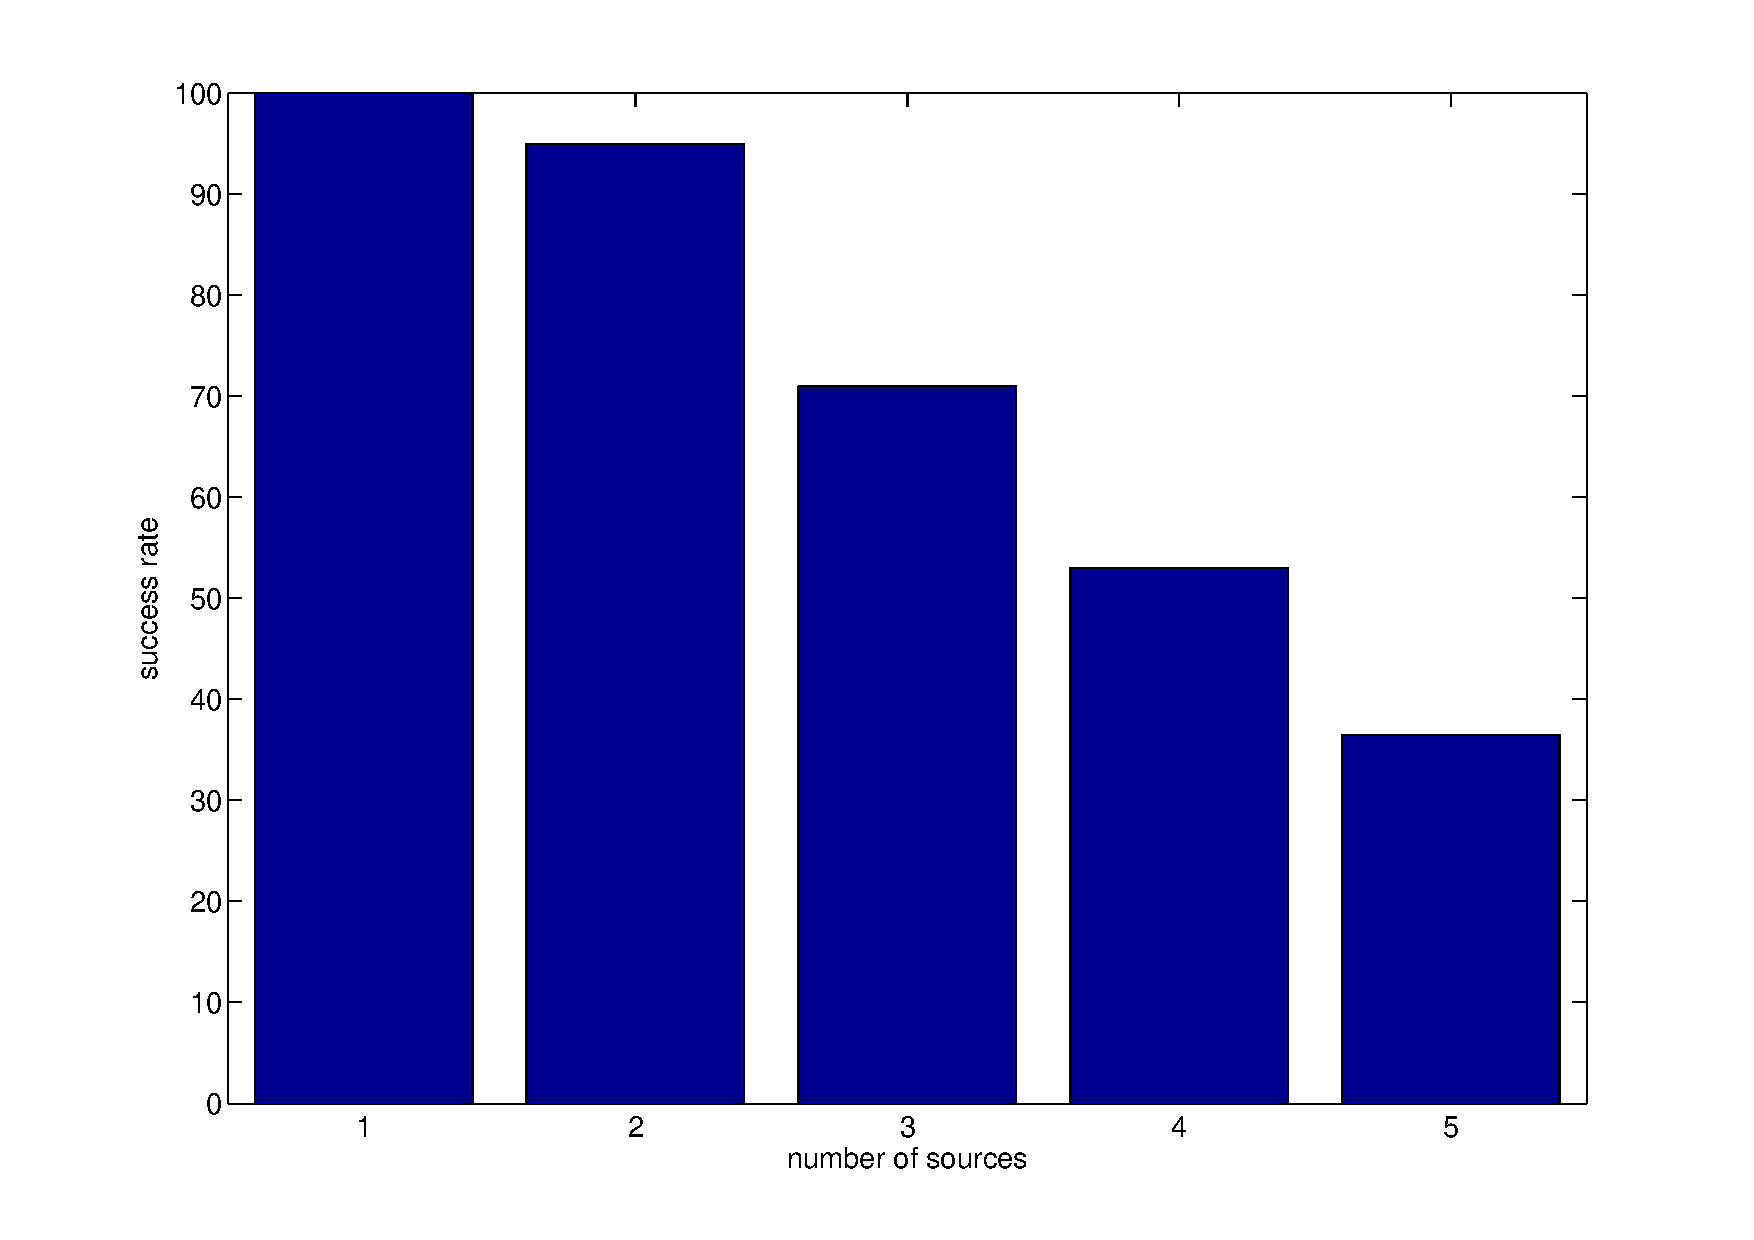
\includegraphics[width=0.8\columnwidth]{images/success_one_mic.pdf}%
%\caption{Average success rate of localization using one microphone.}%
%\label{onemicgauss}%
%\end{figure}